% !TeX root = er.tex

\chapter{Unités de mesure}\label{ch.units}
\index{unités de mesure}

Les tableaux~\ref{tab.units} et \ref{tab.prefixes} présentent les unités de mesure et leurs abréviations.

\begin{table}
\caption{Unités de mesure}
\label{tab.units}
\begin{tabular}{p{2cm}p{1.5cm}p{2.5cm}p{2cm}}
\hline
Propriété & Variable & Unité & Abréviation \\
\hline
Distance & $s$ & mètre & m\\
Temps & $t$ & seconde & s\\
Vélocité & $v$ & mètre/seconde & m/s\\
Accélération & $a$ & mètre/seconde$^2$ & m/s$^2$\\
Fréquence & $f$ & hertz& Hz\\
Angle & $\theta$ & radian & rad\\
& degré & $^\circ$\\
\hline
\end{tabular}
\end{table}

\begin{table}
\caption{Prefixes}
\label{tab.prefixes}
\begin{tabular}{p{1.5cm}p{2.2cm}p{1.7cm}}
\hline
Préfixe & signification & abréviation \\
\hline
kilo- & millièmes & k\\
centi- & centièmes & c\\
milli- & millièmes & m\\
micro & millionièmes & $\mu$\\
\hline
\end{tabular}
\end{table}

\noindent\textbf{Exemples:}

\begin{itemize}\setlength{\itemsep}{6pt}
\item $20$ kHz $=$ $20$ kilohertz $=$ $20,000$ hertz
\item $15$ cm $=$ $15$ centimeters $=$ $\frac{15}{100}$ meters
\item $50$ ms $=$ $50$ milliseconds $=$ $\frac{50}{1000}$ seconds
\item $10$ $\mu$s $=$ $10$ microseconds $=$ $\frac{10}{1000}$ milliseconds $=$ $\frac{10}{1000000}$ seconds
\end{itemize}

Angles, such as the heading of a robot and the direction to an object, are measured in degrees or radians (Fig.~\ref{fig.angles}). By convention, angles are positive in the counterclockwise direction and negative in the clockwise direction as measured from the front of the robot.

\begin{figure}
\begin{center}
% The unit circle divided into 45 degree segments
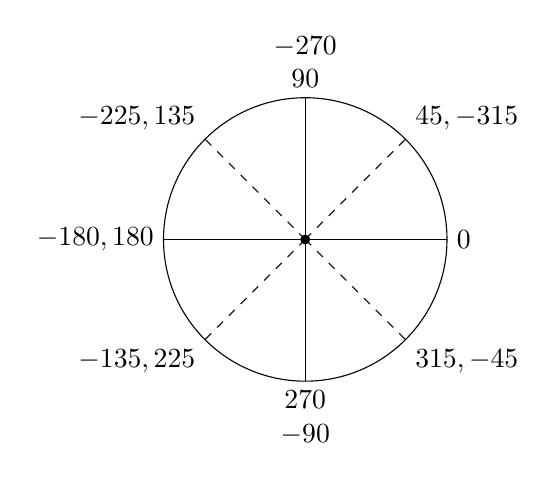
\begin{tikzpicture}[scale=1.8]
\coordinate (origin) at (0,0);
% Draw circle
\draw (origin) circle [radius=1];
% Draw axes
\draw (-1,0) node [left] {$-180,180$} -- (1,0) node [right] {$0$};
\draw (0,-1) node [below,align=flush center] {$270$\\$-90$} -- (0,1) node [above,align=flush center] {$-270$\\$90$};
% Draw other angles
\draw[dashed] (origin) -- +(45:1) node[above right] {$45,-315$};
\draw[dashed] (origin) -- +(135:1) node[above left] {$-225,135$};
\draw[dashed] (origin) -- +(225:1) node[below left] {$-135,225$};
\draw[dashed] (origin) -- +(315:1) node[below right] {$315,-45$};
% Dot at origin
\fill (origin) circle [radius=1pt];
\end{tikzpicture}
\hspace{\fill}
% The unit circle with radians divided into pi/4 segments
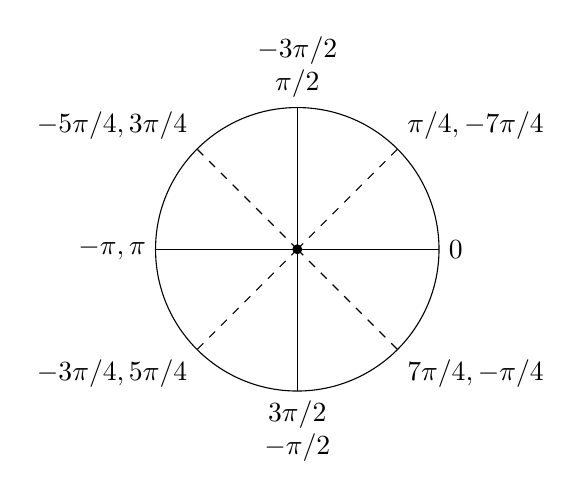
\begin{tikzpicture}[scale=1.8]
\coordinate (origin) at (0,0);
% Draw circle
\draw (origin) circle [radius=1];
% Draw axes
\draw (-1,0) node [left] {$-\pi,\pi$} -- (1,0) node [right] {$0$};
\draw (0,-1) node [below,align=flush center] {$3\pi/2$\\$-\pi/2$} -- (0,1) node [above,align=flush center] {$-3\pi/2$\\$\pi/2$};
% Draw other angles
\draw[dashed] (origin) -- +(45:1) node[above right] {$\pi/4,-7\pi/4$};
\draw[dashed] (origin) -- +(135:1) node[above left] {$-5\pi/4,3\pi/4$};
\draw[dashed] (origin) -- +(225:1) node[below left] {$-3\pi/4,5\pi/4$};
\draw[dashed] (origin) -- +(315:1) node[below right] {$7\pi/4,-\pi/4$};
% Dot at origin
\fill (origin) circle [radius=1pt];
\end{tikzpicture}
\end{center}
\caption{Angles en degrés (à gauche) et en radians (à droite)}\label{fig.angles}
\end{figure}

\chapter{Dérivations mathématiques et tutoriels}\label{ch.math}

Cette annexe rassemble les dérivations mathématiques utilisées dans le texte ainsi que de courts tutoriels sur des concepts qui peuvent ne pas être familiers.

\section{Probabilité conditionnelle et règle de Bayes}\label{a.bayes}

Compte tenu d'une lecture $z$ du capteur, quelle est la probabilité que nous nous trouvions à la position $x_i$ ? Cette probabilité est exprimée sous la forme d'une \emph{probabilité conditionnelle}\index{probabilité!conditionnelle} $p(x_i\mid z)$. Les données dont nous disposons sont la probabilité \emph{actuelle} $p(x_i)$ que nous nous trouvons à $x_i$, et $p(z\mid x_i)$, la probabilité conditionnelle que le capteur lise $z$ si nous nous trouvons en fait à $x_i$. Multiplions ces deux probabilités :
\[
p(z\mid x_i)\, p(x_i)\,.
\]
Qu'est-ce que cela signifie ? L'événement $x_i$ se produit avec la probabilité $p(x_i)$ et une fois qu'il s'est produit, l'événement $z$ se produit avec la probabilité $p(z\mid x_i)$. Il s'agit donc de la probabilité que $z$ et $x_i$ se produisent, appelée \emph{probabilité conjointe}\index{probabilité!conjointe} des deux événements :
\[
p(z \cap x_i) = p(z\cap x_i)\, p(x_i)\,.
\]
La probabilité conjointe peut également être obtenue en multipliant la probabilité conditionnelle de $x_i$ étant donné $z$ par la probabilité de $z$ :
\[
p(x_i \cap z) = p(x_i\mid z)\, p(z)\,.
\]
La probabilité conjointe est commutative, donc en égalant les deux expressions, nous avons :
\[
p(x_i \mid z) = p(x_i \cap z) = p(z\cap x_i)= p(z|mid x_i)p(x_i),.
\]
En divisant par $p(z)$, on obtient :
\[
p(x_i\mid z)= \frac{p(z\mid x_i)\, p(x_i)}{p(z)}\,,
\]
ce qui est connu sous le nom de \emph{règle de Bayes}\index{probabilité!règle de Bayes}.

Si nous connaissons $p(z\mid x_i)$ et $p(x_i)$ pour chaque $i$, $p(z)$, la \emph{probabilité totale} de l'événement $z$, peut être calculée en additionnant les probabilités individuelles connues :
\begin{displaymath}
p(z) = \sum_i p(z\mid x_i)\, p(x_i)\,.
\end{displaymath}

\noindent\textbf{Exemple} Faisons le calcul pour l'exemple de la Sect.~\ref{s.prob-local}. Soit $x_i$ l'événement que nous sommes à la position $i$ et $z$ l'événement que le robot détecte une porte. Initialement, $p(x_i)=.125$ pour toutes les positions $x_i$, et, si le robot se trouve devant une porte, la probabilité que le capteur la détecte correctement est de $.9$, tandis que la probabilité qu'il détecte incorrectement une porte est de $1-.9=.1$. La probabilité de détecter une porte, $p(z)$, est obtenue en additionnant les probabilités à chaque position, où la probabilité est de $.125 fois 0.9 = .1125$ à une position avec une porte et $.125 fois .1= .0125$ à une position sans porte :
\[
p(z)= .1125 + .1125 + .0125 + .0125 + .1125 + .1125 + .1125 + .0125 = .575\,.
\]
Par la règle de Bayes, la probabilité d'être à la position $i$ avec une porte \emph{si} une porte est détectée est :
\[
p(x_i \mid z) = \frac{p(z\mid x_i)\, p(x_i)}{p(z)}=\frac{.9\times .125}{.575} = .196\,,
\]
tandis que la probabilité d'être à la position $i$ sans porte, mais incorrectement une porte est détectée est :
\[
p(x_i \mid z) = \frac{p(z\mid x_i)\, p(x_i)}{p(z)}=\frac{.1\times .125}{.575} = .022\,.
\]

\section{Normalisation}\label{a.normalize}
\index{probabilité!normalisation}

L'ensemble des probabilités des résultats possibles d'un événement doit être égal à $1$ puisque l'un des résultats doit se produire. Si une porte est détectée, le robot doit se trouver à l'une des $8$ positions possibles, mais la somme sur toutes les positions $i$ de la probabilité que le robot se trouve à la position $i$ a été montrée ci-dessus comme étant :
\[
.1125 + .1125 + .0125 + .0125 + .1125 + .1125 + .1125 + .0125 = .575\,.
\]
Les probabilités doivent être \emph{normalisées} en les divisant par la somme $.575$ afin que la somme soit de $1$. Les probabilités normalisées sont $.1125/.575\approx .19$ et $.0125/.575\approx .02$, ce qui donne $1$ :
\[.19 + .19 + .02 + .02 + .19 + .19 + .19 + .02 \approx 1\, .\].

\section{Moyenne et variance}\label{a.mean}

La \emph{moyenne}\index{probabilité!moyenne}\footnote{\textit{Moyenne} est le terme technique pour moyenne.} $\mu$ d'un ensemble de valeurs $\{x_1,\ldots,x_n\}$ est :
\[
\mu = \frac{1}{n}\sum^n_{i=1} x_i\,.
\]
Considérons cinq personnes gagnant respectivement $8,9,10,11,12$ milliers d'euros par an. Leur salaire moyen est de :
\[
\mu = \frac{8+9+10+11+12}{5} = \frac{50}{5} = 10\,.
\]
La moyenne ne nous dit pas grand-chose car la même moyenne peut être obtenue à partir de données très différentes :
\[
\mu = \frac{5+6+10+14+15}{5} = \frac{50}{5} = 10\,.
\]
La moyenne est fortement influencée par les \emph{outliers} : les valeurs qui sont beaucoup plus élevées ou plus basses que le reste des valeurs. Si la personne gagnant $10$ mille euros a soudainement reçu une prime de $90$ mille euros, le salaire moyen est maintenant de :
\[
\mu = \frac{8+9+100+11+12}{5} = \frac{140}{5} = 28\,.
\]
Un politicien sauterait sur l'occasion pour affirmer que, durant son mandat, le salaire moyen a augmenté de $180$ !

\emph{Variance}\index{probabilité!variance} est une mesure de la dispersion d'un ensemble de valeurs. Plus les valeurs sont proches les unes des autres, plus la variance est faible. Les mesures telles que la moyenne sont plus fiables si les valeurs sont regroupées et ont donc une faible variance. La formule de la variance d'un ensemble de valeurs $\{x_1,\ldots,x_n\}$ est la suivante : \footnote{$n-1$ compte les \emph{degrés de liberté}. Comme la moyenne est calculée avant la variance, nous ne pouvons pas choisir les $n$ valeurs arbitrairement ; la dernière valeur choisie est contrainte d'être la valeur qui fait que le calcul produit la moyenne donnée.}
\[
s^2 = \frac{1}{n-1}\sum^n_{i=1} (x_i-\mu)^2\,.
\]
Chaque terme $x_i-\mu$ mesure la distance de la valeur $x_i$ par rapport à la moyenne ; la variance est la moyenne des carrés de ces distances. Les distances sont élevées au carré afin que les valeurs situées de part et d'autre de la moyenne ne s'annulent pas. Par exemple, pour des valeurs de $100$ et $300$, la moyenne est de $200$ ; si nous calculons la variance comme $(100-200)+(200-300)$, le résultat sera de $0$ même si les valeurs sont réparties. En utilisant la définition ci-dessus, la variance est $(100-200)^2+(200-300)^2=20000$.

Pour l'ensemble de données $\{8,9,10,11,12\}$ la variance est :
\[
s^2 = \frac{(-2)^2+(-1)^2+0+1^2+2^2}{5-1} = \frac{10}{4} = 2.5\,,
\]
tandis que pour l'ensemble de données $\{5,6,10,14,15\}$ la variance est :
\[
s^2 = \frac{(-5)^2+(-4)^2+0+4^2+5^2}{4} = 20.5\,.
\]
Comme $20.5$ est beaucoup plus grand que $2.5$, les données de la deuxième série sont réparties sur une plage plus large que les données de la première série. Après réception du bonus, la variance est de :
\[
s^2 = \frac{20^2+19^2+72^2+17^2+16^2}{4} = \frac{6490}{4} = 1622.5\,.
\]
Il est clair qu'il ne faut pas interpréter le salaire moyen comme significatif s'il existe des valeurs aberrantes.

\section{Covariance}\label{a.covariance}
\index{probabilité!covariance}

Considérons un groupe de dix personnes percevant les salaires suivants :
\[x_1=\{11,12,13,14,15,16,17,18,19,20\}\,,
\]
en milliers d'euros. Le salaire moyen est de :
\[
\mu_1=\frac{1}{10}(11+12+13+14+15+16+17+18+19+20)=15.5\,.
\]
Nous supposons que les personnes ayant des salaires élevés achètent des voitures plus chères que celles ayant des salaires faibles. Supposons que deux modèles de voitures soient vendus dans cette zone, l'un pour $10$ mille euros et l'autre pour $20$ mille euros. L'ensemble de données suivant montre les voitures achetées par ce groupe de personnes, où le $i$'th élément est le coût de la voiture achetée par la $i$'th personne :
\[
x_2=\{10,10,10,20,10,20,10,10,20,20\}\,.
\]
Pour voir s'il existe un lien entre les salaires et les coûts des voitures, on calcule la \emph{covariance} $\textit{cov}(x_1,x_2)$ entre les ensembles de données $x_1$ et $x_2$. Le calcul est similaire à celui de la variance, sauf qu'au lieu d'élever au carré la différence entre une valeur d'un seul ensemble et la moyenne de cet ensemble, nous multiplions la différence entre une valeur du premier ensemble et sa moyenne par la différence entre une valeur du deuxième ensemble et sa moyenne :
\[
\textit{cov}(x_1,x_2) = \frac{1}{n-1}\sum^n_{i=1} (x_{1,i}-\mu_1)(x_{2,i}-\mu_2)\,.\label{eq.cov}
\]
La covariance des ensembles de valeurs $x_1$ et $x_2$ est de $7,8$, une valeur positive qui indique que les salaires et le coût des voitures augmentent ensemble, c'est-à-dire que les personnes qui gagnent plus d'argent ont tendance à acheter des voitures plus chères. Si les cinq premières personnes achètent des voitures d'une valeur de $10$ et les cinq suivantes des voitures d'une valeur de $20$, la covariance devient $13.9$, ce qui indique un lien plus fort entre le salaire et le coût d'une voiture. Inversement, si les cinq premiers achètent des voitures chères et les cinq suivants des voitures bon marché, la covariance est de $-13,9$, ce qui signifie que plus le salaire augmente, plus le coût d'une voiture diminue. Enfin, si tout le monde achète la même voiture, la covariance est de $0$ et nous concluons, comme prévu, qu'il n'y a pas de lien entre le salaire et la voiture achetée.

La covariance est symétrique car la multiplication des nombres réels est commutative :
\begin{eqnarray*}
\textit{cov}(x_1,x_2) &=& \frac{1}{n-1}\sum^n_{i=1} (x_{1,i}-\mu_1)(x_{2,i}-\mu_2)\\
&=& \frac{1}{n-1}\sum^n_{i=1} (x_{2,i}-\mu_2)(x_{1,i}-\mu_1)\\
&=&\textit{cov}(x_2,x_1)\,.
\end{eqnarray*}

La matrice de covariance combine les variances et les covariances :
\[
\left[ \begin{array}{ll} s^2(x_1) & \textit{cov}(x_1,x_2)\\ \textit{cov}(x_2,x_1)& s^2(x_2)\end{array}\right]\,.
\]
$\textit{cov}(x_1,x_2)=\textit{cov}(x_2,x_1)$, il n'y a donc que trois valeurs différentes dans la matrice.

\section{Multiplication des vecteurs et des matrices}\label{a.matrices}
\index{multiplication matricielle}

La multiplication d'une matrice (bidimensionnelle) $\vec{M}$ par un vecteur $\vec{v}$ donne un nouveau vecteur :
\[
\spacearray
\vec{M}\vec{v}=\left[ \begin{array}{c} a\\c\end{array} \begin{array}{c} b\\d \end{array}\right]\, \left[ \begin{array}{c} x\\y\end{array}\right] = \left[ \begin{array}{c} ax+by\\cx+by\end{array}\right]\,.
\]
La multiplication de deux matrices s'effectue en multipliant les lignes de la matrice gauche séparément avec chaque vecteur colonne de la matrice droite pour obtenir les vecteurs colonnes de la matrice résultante :
\[
\spacearray
\left[ \begin{array}{c} a\\c\end{array} \begin{array}{c} b\\d \end{array}\right]\, \left[ \begin{array}{c} x\\y\end{array} \begin{array}{c} u\\v\end{array}\right] = \left[ \begin{array}{c} ax+by\\cx+dy\end{array} \;\; \begin{array}{c} au+bv\\cu+dv\end{array}\right]\,.
\]
La matrice identité est :
\[
\spacearray
\vec{I}=\left[\begin{array}{c} 1\\0\end{array} \begin{array}{c} 0\\1\end{array}\right]
\]
et il est facile de vérifier que pour toute matrice $\vec{M}$, $\vec{M}\, \vec{I} = \vec{I}\, \vec{M} = \vec{M}$.
Pour une matrice $\vec{M}$, son inverse $\vec{M}^{-1}$ est la matrice qui donne $\vec{I}$ lorsqu'elle est multipliée par $\vec{M}$ :
\[
\spacearray
\vec{M}=\left[ \begin{array}{c} a\\c\end{array} \begin{array}{c} b\\d \end{array}\right]\,,\;\;\;\;
\vec{M}^{-1}=\frac{1}{\textit{det}\,(\vec{M})}\left[ \begin{array}{c} d\\-c\end{array} \begin{array}{c} -b\\a \end{array}\right]\,,
\]
où $\textit{det}\,(\vec{M})$, le \emph{déterminant} de $\vec{M}$, est $ad-bc$. On peut le vérifier en multipliant :
\[
\spacearray
\left[ \begin{array}{c} a\\c\end{array} \begin{array}{c} b\\d \end{array}\right] \cdot
\left[ \begin{array}{c} d\\-c\end{array} \begin{array}{c} -b\\a \end{array}\right] =
\left[ \begin{array}{c} ad-bc\\cd-dc\end{array} \;\;\begin{array}{c} -ab+ba\\-bc+da \end{array}\right] =
\left[ \begin{array}{c}ad-bc \\0\end{array}\;\; \begin{array}{c} 0\\ad-bc \end{array}\right]\,.
\]
Ceci n'est valable que pour les matrices dont le déterminant est non nul, car les matrices \emph{singular} - celles dont le déterminant est nul - n'ont pas d'inverse.

\section{L'aire d'un trapèze à la base d'un triangle}\label{a.trap}
\index{trapézoïde}

Le diagramme suivant montre un triangle de largeur $w$ et de hauteur $h$ avec une ligne parallèle à la hauteur $h'$ qui crée un trapèze :

\begin{center}
% Computing the area from the uncertainty
\begin{tikzpicture}[scale=1.3]
\draw (0,0) -- (1.5,3) -- (3,0) -- node[below] {$w$} cycle;
\draw (.5,1) -- node[below] {$w'$} (2.5,1);
\draw[<->] (-.4,0) -- node[left] {$h$} (-.4,3);
\draw[<->] (3.4,0) -- node[right] {$h'$} (3.4,1);
\draw[<->] (3.4,1) -- node[right] {$h-h'$} (3.4,3);
\end{tikzpicture}
\end{center}

On veut trouver une formule pour l'aire du trapèze en utilisant les valeurs $w, h, h'$. L'aire $a$ est la différence entre les aires des deux triangles :
\begin{displaymath}
a = \frac{wh}{2} - \frac{w'(h-h')}{2}\,.
\end{displaymath}
Par triangles semblables :
\begin{displaymath}
\frac{h}{h-h'} = \frac{w}{w'}\,,
\end{displaymath}
donc :
\begin{displaymath}
w' = \frac{w(h-h')}{h}\,.
\end{displaymath}
Substitution :
\begin{eqnarray*}
a &=& \frac{wh}{2} - \frac{w(h-h')(h-h')}{2h}\\[8pt]
&=&\frac{w(h^2-(h-h')^2)}{2h}\\[8pt]
&=&\frac{w(h^2-h^2+2hh'-h'^2)}{2h}\\[8pt]
&=&\frac{w(2hh'-h'^2)}{2h}\\[8pt]
&=&wh'(1-\frac{h'}{2h})\,.
\end{eqnarray*}

\section{Formules algébriques pour $\cos 15^{\circ}$}\label{a.cosine}

Eq.~\ref{eq.cos15} affirme que :
\[
\cos^{-1}\left(\frac{\sqrt{2+\sqrt{3}}}{2}\right) = \pm 15^{\circ}\,.
\]
En utilisant la formule du cosinus de la différence de deux angles, nous avons :
\begin{eqnarray*}
\cos 15^\circ &=& \cos(45^\circ-30^\circ)\\
&=& \cos 45^\circ \cos 30^\circ + \sin 45^\circ \sin 30^\circ\\
&=&\frac{\sqrt{2}}{2}\cdot \frac{1}{2} + \frac{\sqrt{2}}{2}\cdot \frac{\sqrt{3}}{2}\\
&=&\frac{\sqrt{2}+\sqrt{6}}{4}\,.
\end{eqnarray*}
Nous calculons maintenant :
\[
\left(\frac{\sqrt{2}+\sqrt{6}}{4}\right)^2 =
\left(\frac{8+2\sqrt{2}\sqrt{6}}{16}\right)=\frac{2+\sqrt{3}}{4}=
\left(\frac{\sqrt{2+\sqrt{3}}}{2}\right)^2\,.
\]
